%%%
%%% BACHELOR'S THESIS TEMPLATE - ENGLISH
%%%  
%%%  * the master file
%%%
%%%  This template requites compilation by the sequence
%%%    latex -> bibtex -> latex (2x) -> dvips -> ps2pdf
%%%  cslatex can be used instead of latex
%%%  pdflatex or pdfcslatex can be used if certain parts are adjusted
%%%
%%%  AUTHORS:  Martin Mares (mares@kam.mff.cuni.cz)
%%%            Arnost Komarek (komarek@karlin.mff.cuni.cz), 2011
%%%            Michal Kulich (kulich@karlin.mff.cuni.cz), 2013
%%%
%%%  LAST UPDATED: 20130318
%%%  
%%%  ===========================================================================

%%%%% Single page layout:
%%%%% ----------------------------------------------------
\documentclass[12pt, a4paper]{report}
\setlength\textwidth{145mm}
\setlength\textheight{247mm}
\setlength\oddsidemargin{15mm}
\setlength\evensidemargin{15mm}
\setlength\topmargin{0mm}
\setlength\headsep{0mm}
\setlength\headheight{0mm}
\let\openright=\clearpage


%%%%% Double page layout
%%%%% ----------------------------------------------------
% \documentclass[12pt, a4paper, twoside, openright]{report}
% \setlength\textwidth{145mm}
% \setlength\textheight{247mm}
% \setlength\oddsidemargin{15mm}
% \setlength\evensidemargin{0mm}
% \setlength\topmargin{0mm}
% \setlength\headsep{0mm}
% \setlength\headheight{0mm}
% \let\openright=\cleardoublepage



%%% Additional useful packages
%%% ----------------------------------------------------------------
\usepackage{amsmath}        
\usepackage{amsfonts}       
\usepackage{amsthm}         
\usepackage{bm}             
\usepackage{graphicx}       
\usepackage{psfrag}         
\usepackage{fancyvrb}       
\usepackage[round]{natbib}         
\usepackage{bbding}         
\usepackage{dcolumn}        
\usepackage{booktabs}       
\usepackage{paralist}       
\usepackage{indentfirst}    
\usepackage[nottoc]{tocbibind}

\usepackage[unicode]{hyperref}
\hypersetup{pdftitle=Thesis Title, 
            pdfauthor=Name Surname,
            ps2pdf,
            colorlinks=false,
            urlcolor=blue,
            pdfstartview=FitH,
            pdfpagemode=UseOutlines,
            pdfnewwindow,
            breaklinks
          }



%%% -------------------------------------
\newcommand{\FIGDIR}{./Obrazky}    %%% directory containing figures


\theoremstyle{plain}
\newtheorem{veta}{Theorem}
\newtheorem{lemma}[veta]{Lemma}
\newtheorem{tvrz}[veta]{Proposition}

\theoremstyle{plain}
\newtheorem{definice}{Definition}

\theoremstyle{remark}
\newtheorem*{dusl}{Corollary}
\newtheorem*{pozn}{Note}
\newtheorem*{prikl}{Example}


\newenvironment{dukaz}{
  \par\medskip\noindent
  \textit{Proof}.
}{
\newline
\rightline{\SquareCastShadowBottomRight}
}


\bibliographystyle{plainnat}     %% Author (year) style
%\bibliographystyle{unsrt}        %% [number] style


%%%%% ------------------------------------------------------------
\DefineVerbatimEnvironment{PCinout}{Verbatim}{fontsize=\small, frame=single}



\newcommand{\R}{\mathbb{R}}
\newcommand{\N}{\mathbb{N}}

\DeclareMathOperator{\pr}{\textsf{P}}
\DeclareMathOperator{\E}{\textsf{E}\,}
\DeclareMathOperator{\var}{\textrm{var}}
\DeclareMathOperator{\sd}{\textrm{sd}}


\newcommand{\T}[1]{#1^\top}        

\newcommand{\goto}{\rightarrow}
\newcommand{\gotop}{\stackrel{P}{\longrightarrow}}
\newcommand{\maon}[1]{o(n^{#1})}
\newcommand{\abs}[1]{\left|{#1}\right|}
\newcommand{\dint}{\int_0^\tau\!\!\int_0^\tau}
\newcommand{\isqr}[1]{\frac{1}{\sqrt{#1}}}

\newcommand{\pulrad}[1]{\raisebox{1.5ex}[0pt]{#1}}
\newcommand{\mc}[1]{\multicolumn{1}{c}{#1}}



%%%%% Main document
%%%%% ---------------------

\begin{document}


%%%
%%% BACHELOR'S THESIS TEMPLATE - ENGLISH
%%%  
%%%  * the title page and front matter
%%%
%%%  AUTHORS:  Martin Mares (mares@kam.mff.cuni.cz)
%%%            Arnost Komarek (komarek@karlin.mff.cuni.cz), 2011
%%%            Michal Kulich (kulich@karlin.mff.cuni.cz), 2013
%%%
%%%  LAST UPDATED: 20130318
%%%  
%%%  ===========================================================================

\pagestyle{empty}
\begin{center}

{\large Charles University in Prague}

\medskip
{\large Faculty of Mathematics and Physics}

\vfill
{\bfseries\Large BACHELOR THESIS}

\vfill
\centerline{\mbox{
\includegraphics[width=60mm]{\FIGDIR/mfflogo.eps}}}

\vfill
\vspace{5mm}

{\LARGE First and last name of the author}

\vspace{15mm}

% Title in English according to the official assignment
{\LARGE\bfseries Title of the thesis}

\vfill

Name of the department or institute
%%% department that confirmed the assignment of the thesis 
%%% according to the Internal Structure of MFF UK in English 
%%% see http://www.mff.cuni.cz/toUTF8.en/fakulta/struktura/sekcem.htm
% Department of Algebra
% Department of Mathematics Education
% Department of Mathematical Analysis
% Department of Numerical Mathematics
% Department of Probability and Mathematical Statistics
% Mathematical Institute of Charles University

\vfill

\begin{tabular}{rl}
Supervisor of the bachelor thesis: & RNDr. Name Surname, Ph.D. \\   
\noalign{\vspace{2mm}}
Study programme: & Mathematics\\
\noalign{\vspace{2mm}}
Specialization: & Specialization\\
%Specialization: & General Mathematics\\
%Specialization: & Financial Mathematics\\
%Specialization: & Mathematical Methods of Information Security\\
\end{tabular}

\vfill

% Fill the year
Prague 2013

\end{center}


%%% At this place, the printed version includes a page containing the
%%% photocopy of the official signed "Bachelor thesis assignment".
%%% This should not be included in the electronic version. 


%%% Acknowledgments
\newpage
\openright

\noindent
I thank \dots\ for \dots. (Not required.)




\newpage
%%% Page containing a legal statement
\vspace*{\stretch{8}}

\noindent
I declare that I carried out this bachelor thesis independently, and only with the cited
sources, literature and other professional sources.

\medskip\noindent
I understand that my work relates to the rights and obligations under the Act No.
121/2000 Coll., the Copyright Act, as amended, in particular the fact that the Charles
University in Prague has the right to conclude a license agreement on the use of this
work as a school work pursuant to Section 60 paragraph 1 of the Copyright Act.

\vspace{18mm}
\noindent
%% Place and date of signature
In \makebox[4cm]{\dotfill} on \makebox[2.5cm]{\dotfill}
\hspace*{\fill}
Author signature
\hspace*{\fill}

\vspace*{\stretch{1}}



\newpage
%%% Czech and English abstracts

\vbox to 0.5\vsize{
\setlength\parindent{0mm}
\setlength\parskip{5mm}

N\'azev pr\'ace:
Czech title according to SIS

Autor:
First and last name of the author

Katedra:  
Czech name of the department or institute
%%% department that confirmed the assignment of the thesis 
%%% according to the Internal Structure of MFF UK in Czech 
%%% see http://www.mff.cuni.cz/toUTF8.cs/fakulta/struktura/sekcem.htm
% Katedra algebry
% Katedra didaktiky matematiky
% Katedra matematick\'e anal\'yzy
% Katedra numerick\'e matematiky
% Katedra pravd\v{e}podobnosti a~matematick\'e statistiky
% Matematick\'y \'ustav UK

Vedouc\'\i\ bakal\'a\v{r}sk\'e pr\'ace:
RNDr. Name Surname, Ph.D., department
%%% First and last name of supervisor with academic titles
%%% Supervisor's department at MFF UK according to the Internal Structure in Czech 
%%% see http://www.mff.cuni.cz/toUTF8.cs/fakulta/struktura/sekcem.htm
%%% Alternatively, full name of external supervisor's institution in Czech
% Katedra algebry
% Katedra didaktiky matematiky
% Katedra matematick\'e anal\'yzy
% Katedra numerick\'e matematiky
% Katedra pravd\v{e}podobnosti a~matematick\'e statistiky
% Matematick\'y \'ustav UK

Abstrakt:
The abstract in Czech, 80\,--\,200 words long, not a copy of the assignment.

Kl\'{\i}\v{c}ov\'a slova:
3 to 5 Czech keywords

\vss}

\nobreak\vbox to 0.49\vsize{
\setlength\parindent{0mm}
\setlength\parskip{5mm}

Title:
English title according to the thesis assignment

Author:
First and last name of the author

Department:
English name of the department or institute
%%% department that confirmed the assignment of the thesis 
%%% according to the Internal Structure of MFF UK in English 
%%% see http://www.mff.cuni.cz/toUTF8.en/fakulta/struktura/sekcem.htm
% Department of Algebra
% Department of Mathematics Education
% Department of Mathematical Analysis
% Department of Numerical Mathematics
% Department of Probability and Mathematical Statistics
% Mathematical Institute of Charles University


Supervisor of the bachelor thesis:
RNDr. Name Surname, Ph.D., department
%%% First and last name of supervisor with academic titles
%%% Supervisor's department at MFF UK according to the Internal Structure in English 
%%% see http://www.mff.cuni.cz/toUTF8.en/fakulta/struktura/sekcem.htm
%%% Alternatively, full name of external supervisor's institution in English
% Department of Algebra
% Department of Mathematics Education
% Department of Mathematical Analysis
% Department of Numerical Mathematics
% Department of Probability and Mathematical Statistics
% Mathematical Institute of Charles University

Abstract:
The abstract in English, 80\,--\,200 words long, not a copy of the assignment.

Keywords:
3 to 5 English keywords
\vss}

%%% A page containing the automatically generated contents of the
%%% bachelor thesis. For a mathematical thesis it is allowed to
%%% place the list of tables and abbreviations at the beginning
%%% of the thesis instead of at the end.
\newpage
\openright

\pagestyle{plain}
\setcounter{page}{1}

\tableofcontents


%%%
%%% BACHELOR'S THESIS TEMPLATE - ENGLISH
%%%  
%%%  * the first chapter
%%%
%%%  AUTHORS:  Arnost Komarek (komarek@karlin.mff.cuni.cz), 2011
%%%            Michal Kulich (kulich@karlin.mff.cuni.cz), 2013
%%%
%%%  LAST UPDATED: 20130318
%%%  

\chapter{Typesetting of mathematical text}

This chapter demonstrates a few examples of mathematical text typesetting.

%%%%% ===============================================================================
\section{Basic examples}


A number in the mathematical mode with decimal point: $\pi \doteq 3.141\,592\,653\,589$.

Test on a 5\% level, 95\% confidence interval.

We have $\var(X) = \E X^2 - \bigl(\E X \bigr)^2$.

\section{Mathematical expressions}
Let
\[
\mathbb{X} = \begin{pmatrix}
      \T{\bm x_1} \\
      \vdots \\
      \T{\bm x_n}
      \end{pmatrix}.
\]
Note the period after the matrix. The mathematical text is a part of
the sentence grammar and requires standard punctuation. Expressions
that will be referenced should be numbered:
\begin{equation}\label{eq01:Xmat}
\mathbb{X} = \begin{pmatrix}
      \T{\bm x_1} \\
      \vdots \\
      \T{\bm x_n}
      \end{pmatrix}.
\end{equation}
Expression \eqref{eq01:Xmat} defines matrix $\mathbb{X}$. To achieve
better readability and organization, it is advised to number only those
expressions that are referenced. Do not number all displayed
expressions automatically.

Aligning of expressions into several columns:
\begin{alignat*}{3}
S(t) &= \pr(T > t),    &\qquad t&>0       &\qquad&\text{ (right-continuous),}\\
F(t) &= \pr(T \leq t), &\qquad t&>0       &\qquad&\text{ (right-continuous).}
\end{alignat*}

Two binded equations:
\begin{equation}\label{eq01:FS}
\left.
\begin{aligned}
S(t) &= \pr(T > t) \\[1ex]
F(t) &= \pr(T \leq t)
\end{aligned}
\right\}
\quad t>0 \qquad \text{(right-continuous).}
\end{equation}

Two centered unnumbered equations:
\begin{gather*}
\bm Y = \mathbb{X}\bm\beta + \bm\varepsilon, \\[1ex]
\mathbb{X} = \begin{pmatrix} 1 & \T{\bm x_1} \\ \vdots & \vdots \\ 1 &
  \T{\bm x_n} \end{pmatrix}.
\end{gather*}
Two centered numbered equations:
\begin{gather}
\bm Y = \mathbb{X}\bm\beta + \bm\varepsilon, \label{eq02:Y}\\[1ex]
\mathbb{X} = \begin{pmatrix} 1 & \T{\bm x_1} \label{eq03:X}\\ \vdots & \vdots \\ 1 &
  \T{\bm x_n} \end{pmatrix}.
\end{gather}

Definition organized by cases:
\[
P_{r-j}=
\begin{cases}
0 & \text{if $r-j$ is odd},\\
r!\,(-1)^{(r-j)/2} & \text{if $r-j$ is even}.
\end{cases}
\]
Note the use of punctuation in the equation. Commas and periods are
placed according to the standard English language rules.

\begin{align}
x& = y_1-y_2+y_3-y_5+y_8-\dots && \text{by \eqref{eq02:Y}} \nonumber\\
& = y'\circ y^* && \text{by \eqref{eq03:X}} \nonumber\\
& = y(0) y' && \text {by Axiom 1.}
\end{align}

Two unnumbered aligned equations:
\begin{align*}
L(\bm\theta) &= \prod_{i=1}^n f_i(y_i;\,\bm\theta), \\
\ell(\bm\theta) &= \log\bigl\{L(\bm\theta)\bigr\} = 
\sum_{i=1}^n \log\bigl\{f_i(y_i;\,\bm\theta)\bigr\}.
\end{align*}
Two aligned equations, the first numbered:
\begin{align}
L(\bm\theta) &= \prod_{i=1}^n f_i(y_i;\,\bm\theta), \label{eq01:L} \\
\ell(\bm\theta) &= \log\bigl\{L(\bm\theta)\bigr\} = 
\sum_{i=1}^n \log\bigl\{f_i(y_i;\,\bm\theta)\bigr\}. \nonumber
\end{align}

Two-line equation, the first line aligned left, the second line
aligned right, unnumbered:
\begin{multline*}
\ell(\mu,\,\sigma^2) = \log\bigl\{L(\mu,\,\sigma^2)\bigr\} = 
\sum_{i=1}^n \log\bigl\{f_i(y_i;\,\mu,\,\sigma^2)\bigr\} \\
  = -\,\frac{n}{2}\,\log(2\pi\sigma^2) \,-\, 
\frac{1}{2\sigma^2}\sum_{i=1}^n\,(y_i - \mu)^2. 
\end{multline*}

Two-line equation, aligned to $=$, numbered in the middle:
\begin{equation}\label{eq01:ell}
\begin{split}
\ell(\mu,\,\sigma^2) &= \log\bigl\{L(\mu,\,\sigma^2)\bigr\} = 
\sum_{i=1}^n \log\bigl\{f(y_i;\,\mu,\,\sigma^2)\bigr\} \\
& = -\,\frac{n}{2}\,\log(2\pi\sigma^2) \,-\, 
\frac{1}{2\sigma^2}\sum_{i=1}^n\,(y_i - \mu)^2. 
\end{split}
\end{equation}


%%%%% ===============================================================================
\section{Definitions, theorems, proofs, \dots}

Constructions like definitions, theorems, examples, \dots, should be
separated from the surrounding  text and (usually) numbered, with the
use of cross-references. For each of these constructions, the main
source file (\texttt{BcPrace.tex}) should define an environment
providing its visual separation from the surrounding text and
numbering/cross-referencing features. 

\begin{definice}\label{def01:1}
  Let random variables $X_1,\dots,X_n$ be defined on the same
  probability space $(\Omega,\,\mathcal{A},\,\pr)$. Then the vector
  $\bm X = \T{(X_1,\dots,X_n)}$ is called a \emph{random
    vector}.
\end{definice}

\begin{definice}[random vector]\label{def01:2}
  Let random variables $X_1,\dots,X_n$ be defined on the same
  probability space $(\Omega,\,\mathcal{A},\,\pr)$. Then the vector
  $\bm X = \T{(X_1,\dots,X_n)}$ is called a \emph{random
    vector}.
\end{definice}
Definition~\ref{def01:1} demonstrates an environment without a
subtitle, definition~\ref{def01:2} includes a subtitle.

\begin{veta}\label{veta01:1}
  The random vector $\bm X$ is a measurable mapping of the space 
  $(\Omega,\,\mathcal{A},\,\pr)$ to $(\R_n,\,\mathcal{B}_n)$.
\end{veta}

\begin{lemma}[\citealp{Andel07}, str. 29]\label{veta01:2}
  The random vector $\bm X$ is a measurable mapping of the space 
  $(\Omega,\,\mathcal{A},\,\pr)$ to $(\R_n,\,\mathcal{B}_n)$.
\end{lemma}
\begin{dukaz}
  The detailed steps of the proof are described in the book \citet[p.
  29]{Andel07}. 
\end{dukaz}
Theorem~\ref{veta01:1} demonstrates an environment without a subtitle,
lemma~\ref{veta01:2} includes a reference in the subtitle. Lemmas were
defined in the main file so that they share the same numbering with
theorems.




%%%
%%% BACHELOR'S THESIS TEMPLATE - ENGLISH
%%%  
%%%  * the second chapter
%%%
%%%  AUTHORS:  Arnost Komarek (komarek@karlin.mff.cuni.cz), 2011
%%%            Michal Kulich (kulich@karlin.mff.cuni.cz), 2013
%%%
%%%  LAST UPDATED: 20130318
%%%  
%%%  ===========================================================================

\chapter{Citations}

Citations are created by commands
\texttt{{\textbackslash}citet}, \texttt{{\textbackslash}citep} etc.
(see {\LaTeX} package \textsf{natbib}) and processed by running
Bib{\TeX}. In mathematical publications, citations are usually
formatted as ``Author name (year of publication)'' or ``Author name
[number of the reference])''. Citations by author name are easier to
handle in English than in Czech, because of its simpler grammar rules.


%%%%% =====================================

\section{Some examples}

\citet{KaplanMeier58, Cox72} belong among the most highly cited statistical papers.
\citet{Student08} wrote a paper on the t-test. 

Prof. And\v{e}l authored a famous textbook on mathematical statistics
\citep[see][]{Andel98}. The theory of estimation is the topic of
\citet{LehmannCasella98}. When a reference to a specific result
(definition, theorem, proof,\ldots) is made it is useful to include the
number of the chapter, page, or theorem in the citation, e.g.,
\citet[Theorem 4.22]{Andel07} or \citep[see][Chapter~4]{Andel07}.

Some papers have many coauthors. When citing a paper with three
coauthors we usually list all of them at the first ocassion:
\citet*{DempsterLairdRubin77} introduced the concept of the EM
algorithm. Alternatively: The concept of the EM algorithm was
introduced in the late seventies \citep*{DempsterLairdRubin77}. When
that same paper is cited again, we use a short citation:
\citet{DempsterLairdRubin77} offer several examples of the use of the
EM algorithm.

Papers with more than three coauthors are always cited in the short form:
The first results from Project ACCEPT were published by 
\citet{Genberget08}. \emph{We never cite this paper as} \citet*{Genberget08}.

%%%
%%% BACHELOR'S THESIS TEMPLATE - ENGLISH
%%%  
%%%  * the third chapter
%%%
%%%  AUTHORS:  Arnost Komarek (komarek@karlin.mff.cuni.cz), 2011
%%%            Michal Kulich (kulich@karlin.mff.cuni.cz), 2013
%%%
%%%  LAST UPDATED: 20130318
%%%  
%%%  ===========================================================================

\chapter{Tables, figures, software code}

The inclusion of tables and figures in a scientific publication follows
certain common and certain specific rules. Tables and figures are not
included inside the text but placed either on dedicated pages or floated
at the top or the bottom of a text page. \LaTeX\ handles floating
figures and tables automatically. Every table and figure must be
numbered and accompanied with a legend. The legend should describe the
contents of the table of figure with enough detail so that the reader
can understand them without studying the text of the publication. Each
table and figure should be refrenced by its number in the text. The
text should summarize the most important conclusions that can be drawn
from the table of figure. The text should be easy to follow and
understand even without seeingf the figures and tables (and on the
contrary, the figures and tables should be easy to understand even
without reading the text). Figures and tables should be referenced
indirectly in the sentences: instead of
\emph{``Table~\ref{tab03:Nejaka} shows that men are on average $9.9$
  kg heavier than women''} we write \emph{``Men are on average $9,9$
  kg heavier than women (see Table~\ref{tab03:Nejaka})}.


%%%%% ===============================================================================
\section{Tables}

\begin{table}[b!]

\centering
%%% The following packages are needed for this example:
%%%   - booktabs (\toprule, \midrule, \bottomrule)
%%%   - dcolumn (column type  D)
%%% Commands \pulrad and \mc defined in BcPrace.tex are used

\begin{tabular}{l@{\hspace{1.5cm}}D{.}{.}{3.2}D{.}{.}{1.2}D{.}{.}{2.3}}
\toprule
 & \mc{} & \mc{\textbf{Std.}} & \mc{} \\
\pulrad{\textbf{Effect}} & \mc{\pulrad{\textbf{Estimate}}} & \mc{\textbf{error}$^a$} & 
\mc{\pulrad{\textbf{P-value}}} \\
\midrule
Intercept     & -10.01 & 1.01 & \mc{---} \\
Gender (male) & 9.89   & 5.98 & 0.098 \\
Height (cm)    & 0.78   & 0.12 & <0.001 \\ 
\bottomrule
\multicolumn{4}{l}{\footnotesize \textit{Note:} 
$^a$ Standard error of the estimator by the Monte Carlo method.}
\end{tabular}

\caption{Maximum likelihood estimates from model M.}\label{tab03:Nejaka}

\end{table}


\textbf{Tables} should be formatted according to the following rules:
\begin{compactitem} %% requires package paralist
\item Avoid vertical lines. Separate the table from the surrounding
  text (even the legend) by stronger horizontal lines. Separate the
  header from the table and different parts of the table from each
  other by thinner horizontal lines. This table format can be obtained
  in \LaTeX\ by loading the package \texttt{booktabs}. If a stronger
  separation of the columns is desired it can be achieved by including
  an additional vertical space. 
\item Do not change the type, format and meaning of the cells in a
  single column (never include means in some cells and percentages in
  other cells of the same column).
\item Do not repeat the same cell contents many times. If the table
  includes the column ``Variance'', which contains the value 0.5 in
  the first ten cells and 1.5 in the next ten cells, delete this
  column and find another way to communicate the value of the
  variance. For example, the table can be divided into two separate
  tables and the variance given in the legend. Or additional rows can
  be included between the parts of the table informing what was the
  variance in the subsequent rows.
\item Numeric columns in the table should be aligned on the decimal
  point. 
\item Tables sometimes include abbreviations that are not used
  elsewhere in the text. These abbreviations should be explained in
  the legend or in notes under the table. These notes can be also used
  to provide more detail on the meaning of selected columns or cells. 
\end{compactitem}




\section{Figures}

Some advice on figures and diagrams:
\begin{compactitem}
\item Create the figure in the same size that will be used in the
  thesis. Excessive magnification or reduction of figures causes poor
  readability.
\item The axes of a graph must be carefully annotated in the same
  language the thesis is written in. Units of measurement (kg,
  minutes, \ldots) should be provided when applicable. When the graph
  plots a function $h(x)$ the axes should be annotated by $x$ a
  $h(x)$. Each axis must have a clearly defined scale (tickmarks, labels).
\item If a two-dimensional scatterplot includes a large number of
  points make sure that the points do not turn into black cloud. If
  the number of points is too large reduce the size of the plotting
  symbol or select a subset of the points. Plots that include
  thousands of points make problems in electronic documents, they
  increase the size too much.
\item If the thesis is to be printed on a black-and-white printer, do
  not use colors. Lines can be distinguished by the type (solid,
  dotted, \ldots), areas can be filled by various shades of grey or 

The meaning of the line types and area shading should be explained in
the legend or directly in the plot.
\end{compactitem}

The command \texttt{{\textbackslash}psfrag} can replace parts of 
\textsf{ps/eps} files (usually annotations in the graphs) by an
arbitrary sequence of \LaTeX\ commands, as the following examples
illustrate. 



\section{Software code}

Software code or computer output (if needed in the thesis) should be
formatted differently from the other text. One option is to use
{\LaTeX} package \texttt{fancyvrb}
(fancy verbatim), which is used to define the environment
\texttt{PCinout} in the master file \texttt{BcPrace.tex}. With this
environment, we can generate the following examples:
\begin{PCinout}
> mean(x)
[1] 158.90
> objekt$mean
[1] 158.90
\end{PCinout}
%$
Smaller font:
\begin{PCinout}[fontsize=\footnotesize]
> mean(x)
[1] 158.90
> objekt$mean
[1] 158.90
\end{PCinout}
%$
No frame:
\begin{PCinout}[frame=none]
> mean(x)
[1] 158.90
> objekt$mean
[1] 158.90
\end{PCinout}
%$
Narrow frame:
\begin{PCinout}[xrightmargin=20em]
> mean(x)
[1] 158.90
> objekt$mean
[1] 158.90
\end{PCinout}
%$


\begin{figure}[p]\centering
\psfrag{x}[c][c]{\textsf{\large horizontal axis ($\mu_1 = 0, \sigma_1^2 = 1$)}}
\psfrag{y}[c][c]{\textsf{\large vertical axis ($\mu_2 = 0, \sigma_2^2 = 1$)}}
\psfrag{Plot}[c][c]{\textsf{\bfseries\Large Scatterplot}}

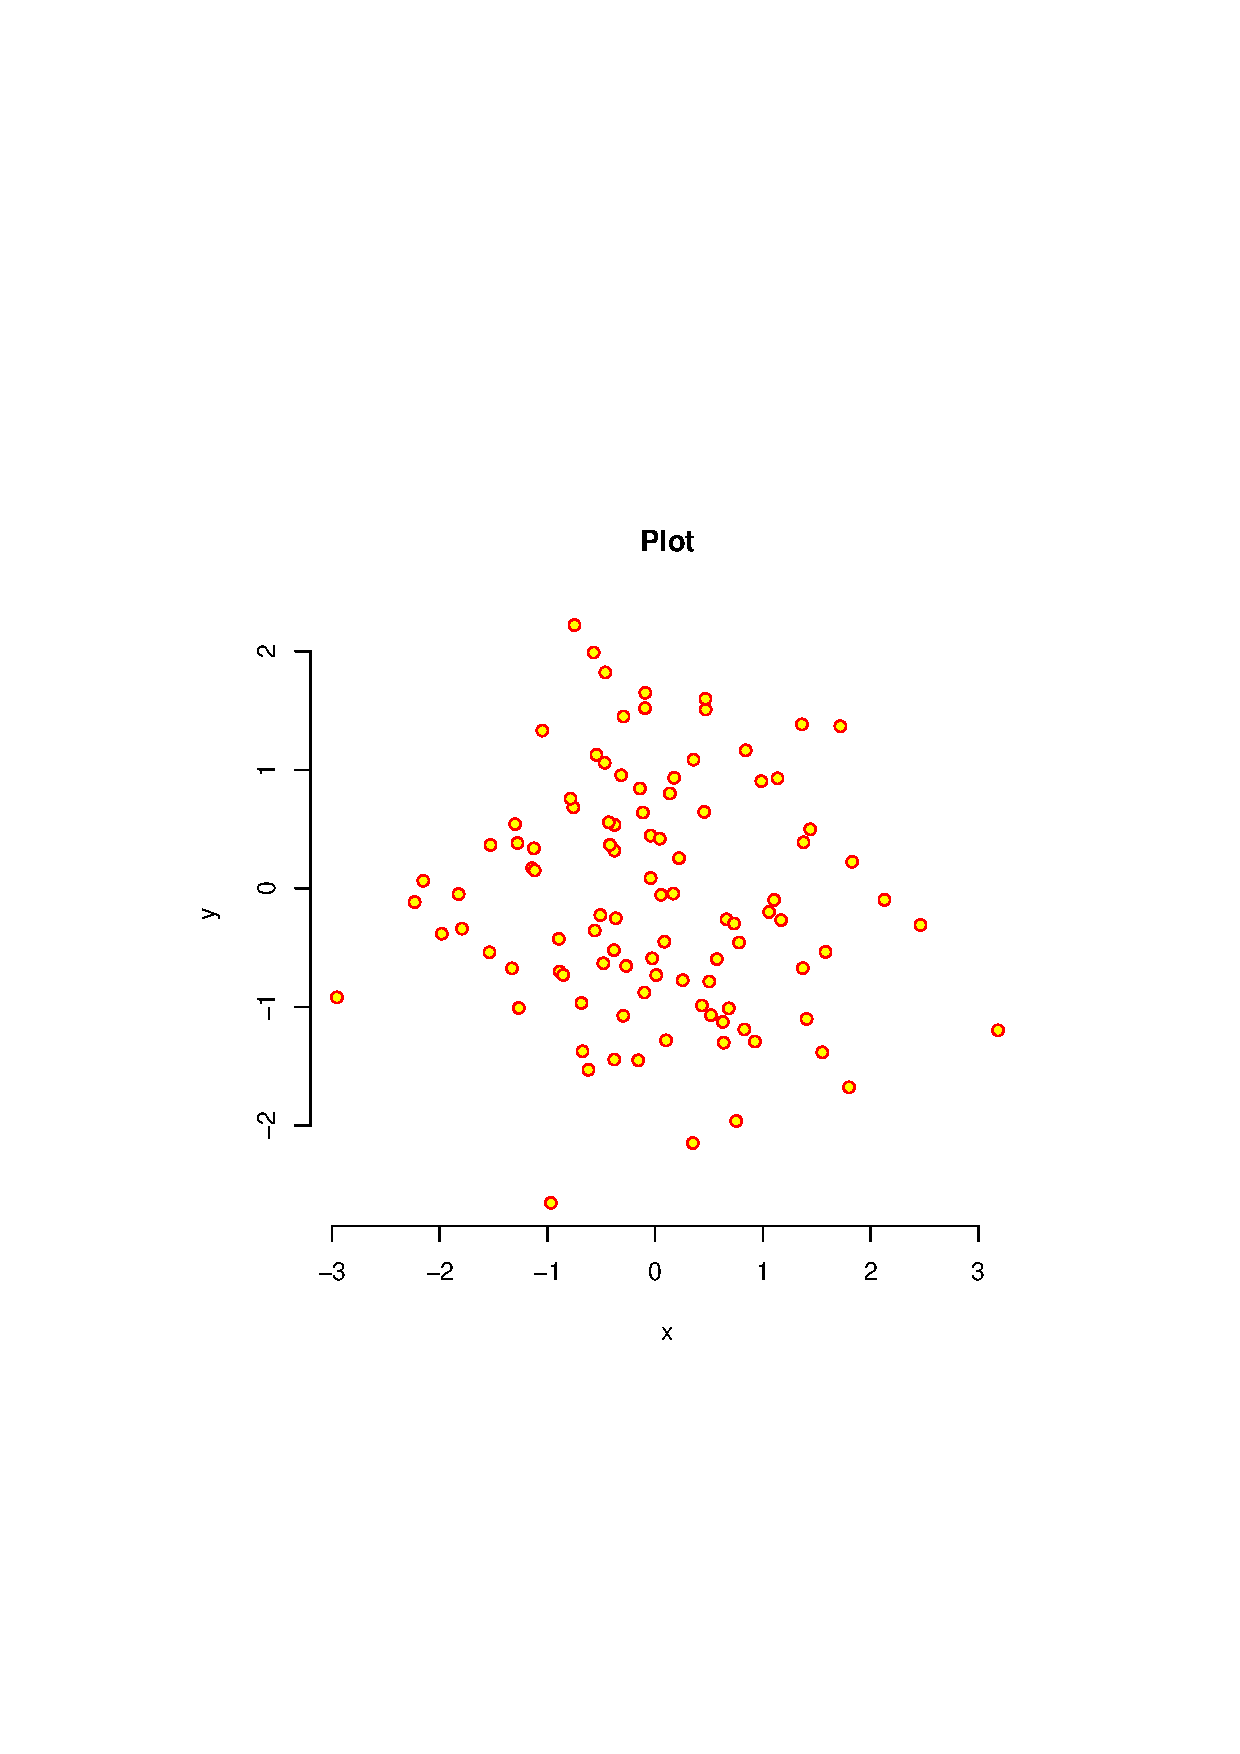
\includegraphics[width=6in, height=6in]{\FIGDIR/obr01}     

\caption{Random sample from distribution $\mathcal{N}_2(\boldsymbol{0},\,I)$.}
\label{obr03:Nvyber}

\end{figure}


\begin{figure}[p]\centering
\psfrag{0.00}[c][c]{\textsf{0{,}00}}  
\psfrag{0.02}[c][c]{\textsf{0{,}02}}  
\psfrag{0.04}[c][c]{\textsf{0{,}04}}
\psfrag{0.06}[c][c]{\textsf{0{,}06}}  
\psfrag{0.08}[c][c]{\textsf{0{,}08}}
\psfrag{m = 100, s = 15}[l][l]{\textsf{\large $\mu = 100,\; \sigma = 15$}}
\psfrag{m = 110, s = 10}[l][l]{\textsf{\large $\mu = 110,\; \sigma = 10$}}
\psfrag{m = 120, s = 5}[l][l]{\textsf{\large $\mu = 120,\; \sigma = 5$}}

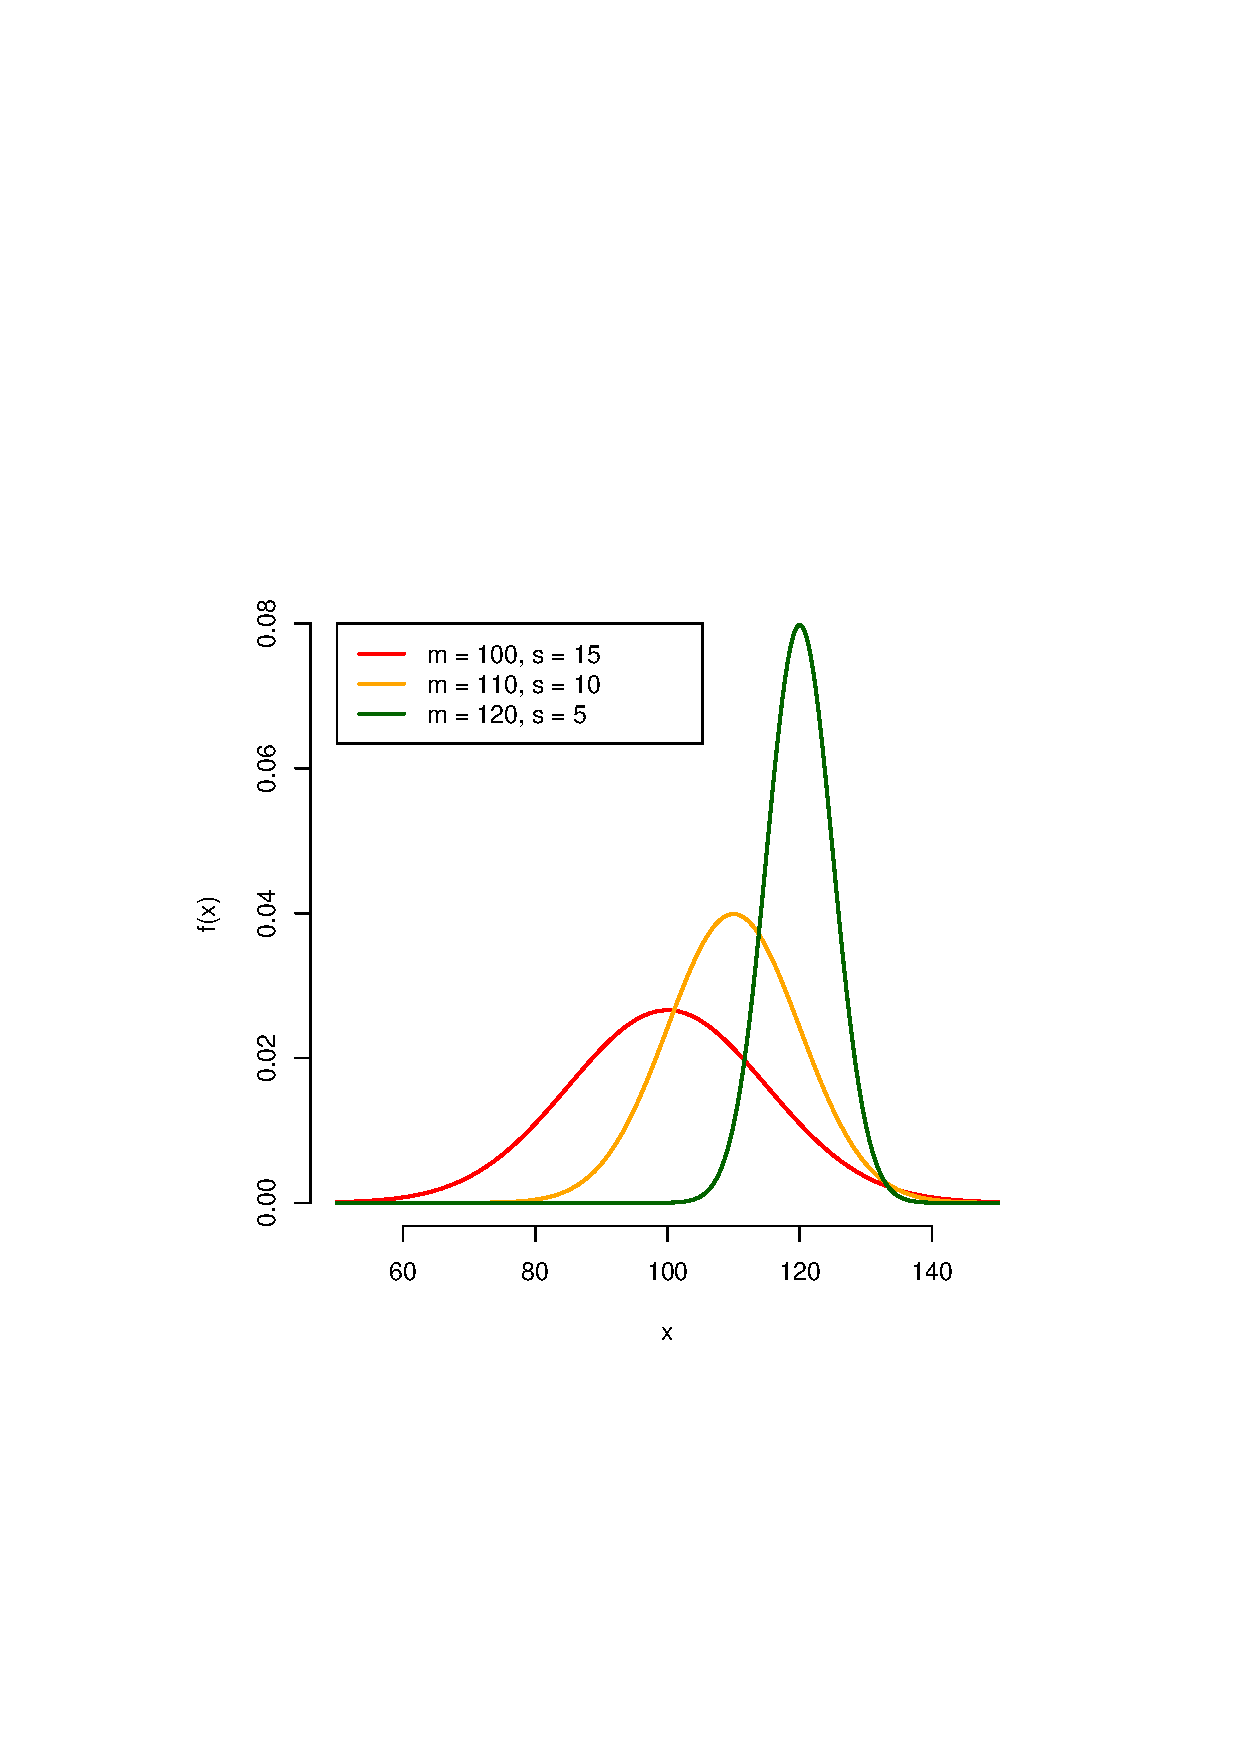
\includegraphics[width=6in, height=6in]{\FIGDIR/obr02}

\caption{Densities of several normal distributions.}
\label{obr03:Nhust}

\end{figure}


\begin{figure}[p]\centering
\psfrag{0.00}[c][c]{\textsf{\small 0{,}00}}  
\psfrag{0.02}[c][c]{\textsf{\small 0{,}02}}  
\psfrag{0.04}[c][c]{\textsf{\small 0{,}04}}
\psfrag{0.06}[c][c]{\textsf{\small 0{,}06}}  
\psfrag{0.08}[c][c]{\textsf{\small 0{,}08}}
\psfrag{60}[c][c]{\textsf{\small 60}}    
\psfrag{80}[c][c]{\textsf{\small 80}}  
\psfrag{100}[c][c]{\textsf{\small 100}}
\psfrag{120}[c][c]{\textsf{\small 120}}  
\psfrag{140}[c][c]{\textsf{\small 140}}
\psfrag{f\(x\)}[c][c]{\textsf{\small f(x)}}      
\psfrag{x}[c][c]{\textsf{\small x}}
\psfrag{m = 100, s = 15}[l][l]{\textsf{\large $\boldsymbol{\mu} \mathbf{\;= 100,}\; \boldsymbol{\sigma} \mathbf{\;= 15}$}}
\psfrag{m = 110, s = 10}[l][l]{\textsf{\large $\boldsymbol{\mu} \mathbf{\;= 110,}\; \boldsymbol{\sigma} \mathbf{\;= 10}$}}
\psfrag{m = 120, s = 5}[l][l]{\textsf{\large $\boldsymbol{\mu}  \mathbf{\;= 120,}\; \boldsymbol{\sigma} \mathbf{\;= 5}$}}

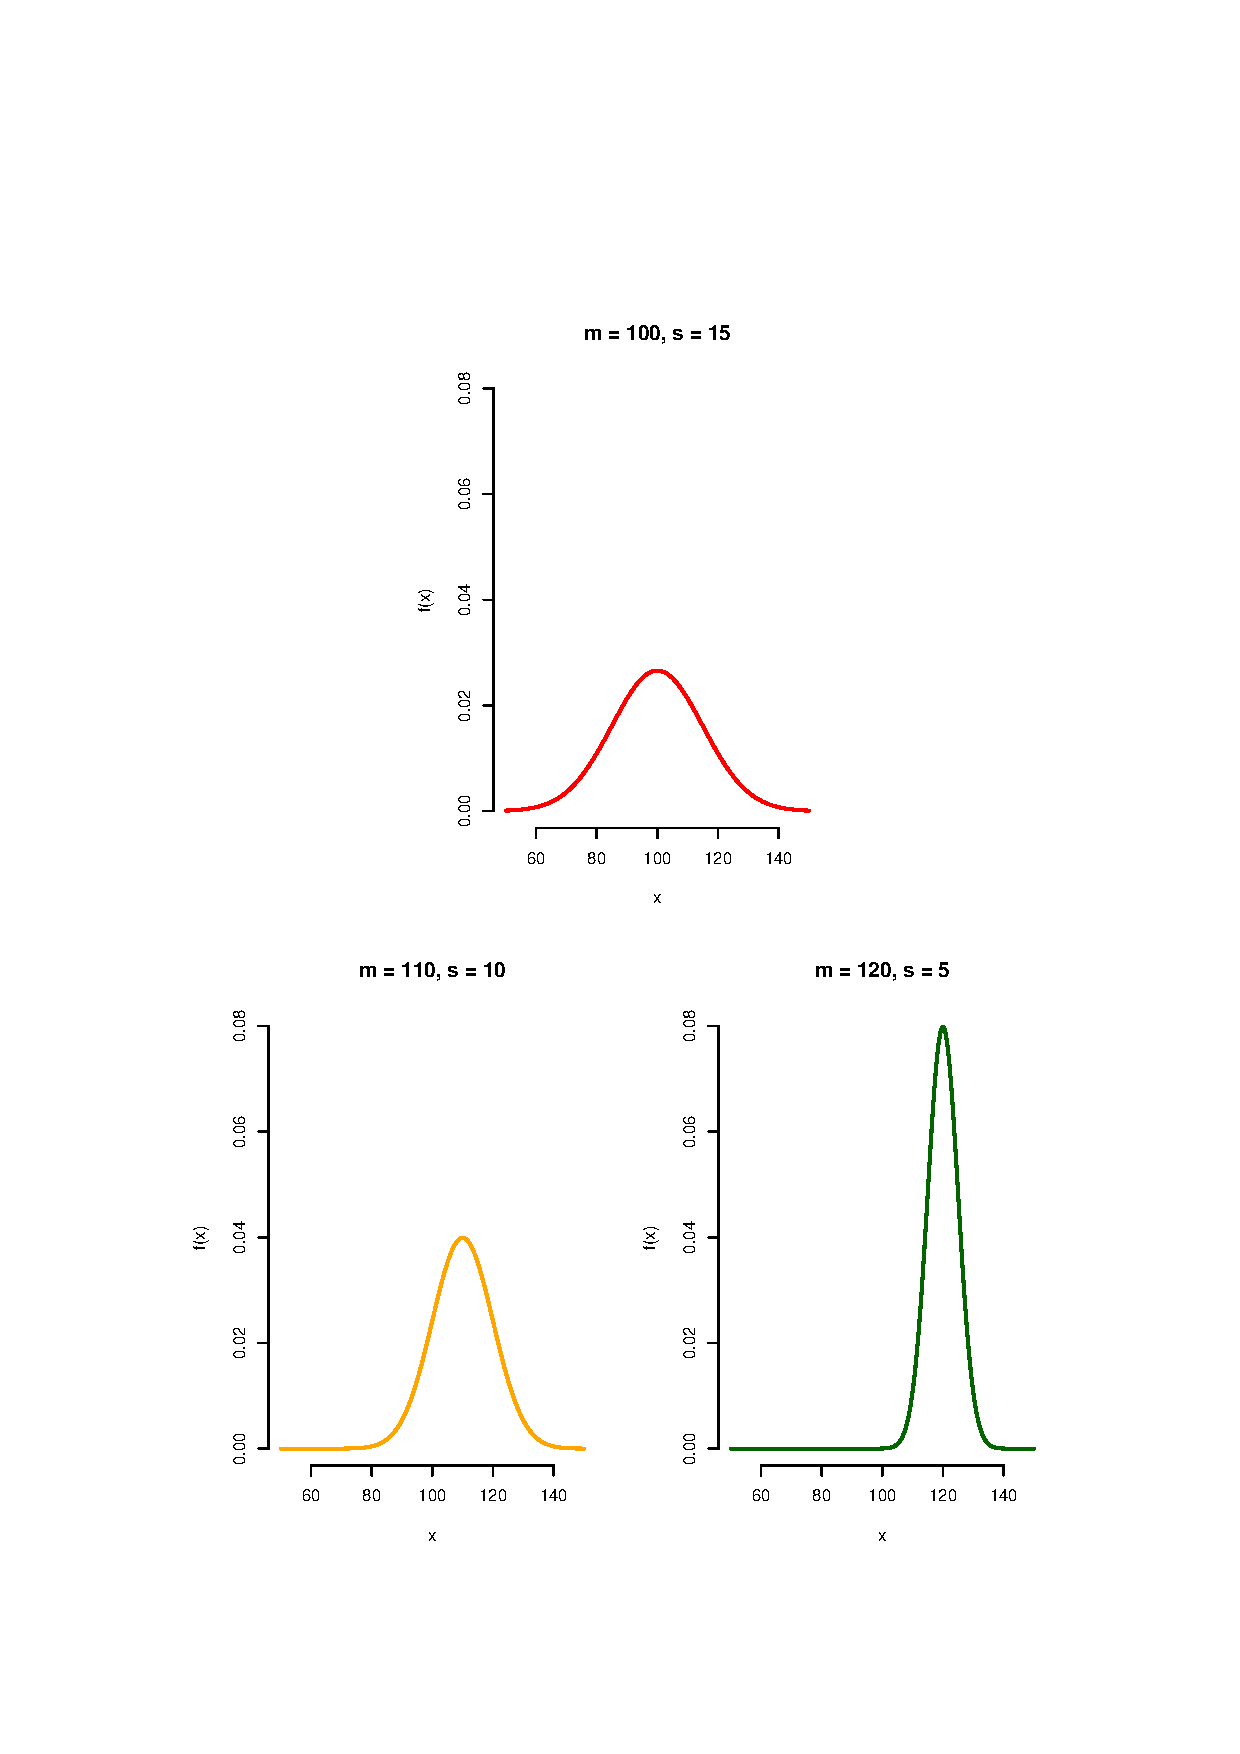
\includegraphics[width=6in, height=8.5in]{\FIGDIR/obr03}

\caption{Densities of several normal distributions.}
\label{obr03:Nhust:podruhe}

\end{figure}



%%% References 
%%% References are sought in the database priklady_literatury.bib.
%%% Requires the compilation sequence latex->bibtex->latex->latex
\bibliography{priklady_literatury}

%%% List of figures
\listoffigures

%%% List of tables
\listoftables

%%% 
%\chapter*{List of abbreviations}
%\addcontentsline{toc}{chapter}{List of abbreviations}


%%% The Appendix. 
%\chapter*{Appendix}
%\addcontentsline{toc}{chapter}{Appendix}



\end{document}

